\FloatBarrier
\subsection{Cooperatively bound tau uniquely interacts with MAPs}
\begin{figure}[h!]
\centering
\includegraphics[width=0.95\linewidth]{Figures/taukatanin.png}
\caption[Tau islands constitute a protective envelope around microtubules.]{
\textbf{Tau islands constitute a protective envelope around microtubules.} (A) Fluorescence micrographs showing katanin-driven (green, example indicated by green arrow) disassembly of Atto-647-microtubules (blue) decorated with tau islands (red, example indicated by red arrow) interspersed by regions of low tau-mEGFP density (indicated by blue arrow). An example region outside an island is indicated by white arrow. An example of an island-covered region being slowly shortened by katanin is indicated by a yellow arrow. (B,C) Boxplots of the velocities of katanin-driven disassembly of stretches of microtubules covered by tau islands (evaluated per island boundary) and the rate of katanin-generated cuts occurring within them, at the two different tested tau concentrations. (E) Exemplary time-traces of normalized tubulin signal outside the island-covered microtubule regions (blue line) decaying during its katanin-driven disassembly. Single exponential fits to the data (black lines) yield a tubulin residence time of 17 ± 6.4 s (average ± S.D., n = 17 microtubules in 2 experiments) in presence of 20 nM tau and 34 ± 23 s (n = 18 microtubules in 2 experiments) in presence of 800 nM tau. Photo-bleaching during this experiment was negligible (Methods). (D) Fluorescence micrographs showing katanin-driven (green) disassembly of Atto-647-microtubules (blue) decorated with tau islands (red) formed at 0.8 µM tau concentration. The island positions (indicated by numbers) were determined via a brief removal of tau from solution. The green arrow shows an example region outside of islands and its decoration with katanin, the red arrow shows an island-covered region (katanin was absent from such regions). An example of rapid disassembly of surrounding regions is indicated by the white arrow. Compare to A. Panels from \cite{Siahaan2019a}.
	}\label{taukatanin}
\end{figure}
To investigate how tau islands interact with other microtubule-associated proteins (MAPs), we formed tau islands and tested the interaction of other axonal MAPs with such tau-decorated microtubules. Among others, we tested the microtubule-transport motor kinesin-1, where we found that while these motors could move freely through surrounding regions, they were totally blocked from accessing island-decorated microtubule regions. However, these experiments were exclusively performed and analzed by my colleague Valerie Siahaan, thus the results for these experiments (see \cite{Siahaan2019a}) are not shown in this thesis. As mentioned in \aref{chap:publications}{}, I contributed to our results regarding the cutting enzyme katanin and was exclusively conducting and analyzing experiments regarding the motor protein kinesin-8.\par

After the addition of 100nM (GFP-labeled) katanin to microtubules in the presence of 20nM (mCherry-labeled) tau, we observed katanin binding almost exclusively to the low-density tau regions surrounding the islands \pref{taukatanin}{A, 15s panel}. As one may expect from this observation, we then subsequently observed microtubule disassembly predominantly in these regions \pref{taukatanin}{A, 30s panel}. Only on longer time scales, the island-covered regions of the microtubules started to disassemble from their boundaries, with occassional cuts occuring inside tau islands \pref{taukatanin}{A-C}. Combined, these results show that tau islands constitute a protective envelope around the microtubule surface, which can hinder the activity of microtubule-severing factors and block kinesin-1-based transport. \par

As shown in the previous section, higher tau concentrations, the tau densities inside and outside tau islands are comparable \pref{tauflushouts}{A}. We thus wondered if the discretely binding tau molecules in the island surroundings, at these concentrations, are sufficient for shielding the microtubule against microtubule severing. We thus formed tau islands at saturating conditions (0.8 µM). After 5 minutes of incubation we briefly removed tau from solution to note the position of the islands, and then again re-introduced 0.8 µM tau in the assay. We then exposed such tau decorated microtubules to 0.2 µM katanin analogously to the experiment presented in \aref{taukatanin}{A}. Strikingly, we observed qualitatively identical results as in \aref{taukatanin}{A}. Namely, regions surrounding the islands and occupied by the diffusible tau phase were severed and rapidly disassembled, while microtubule regions shielded by the islands persisted \pref{taukatanin}{D}. This demonstrates that the density of tau on the microtubule surface is not the factor determining the shielding function of tau. Rather it is the unique nature of the cooperative tau binding mode which protects the microtubules. This conclusion is supported by our observation that increasing the tau concentration in solution did not substantially increase shielding against tau, neither in the island regions \pref{taukatanin}{B,C} nor in their surroundings \pref{taukatanin}{E}.\par

\begin{figure}[h!]
\centering
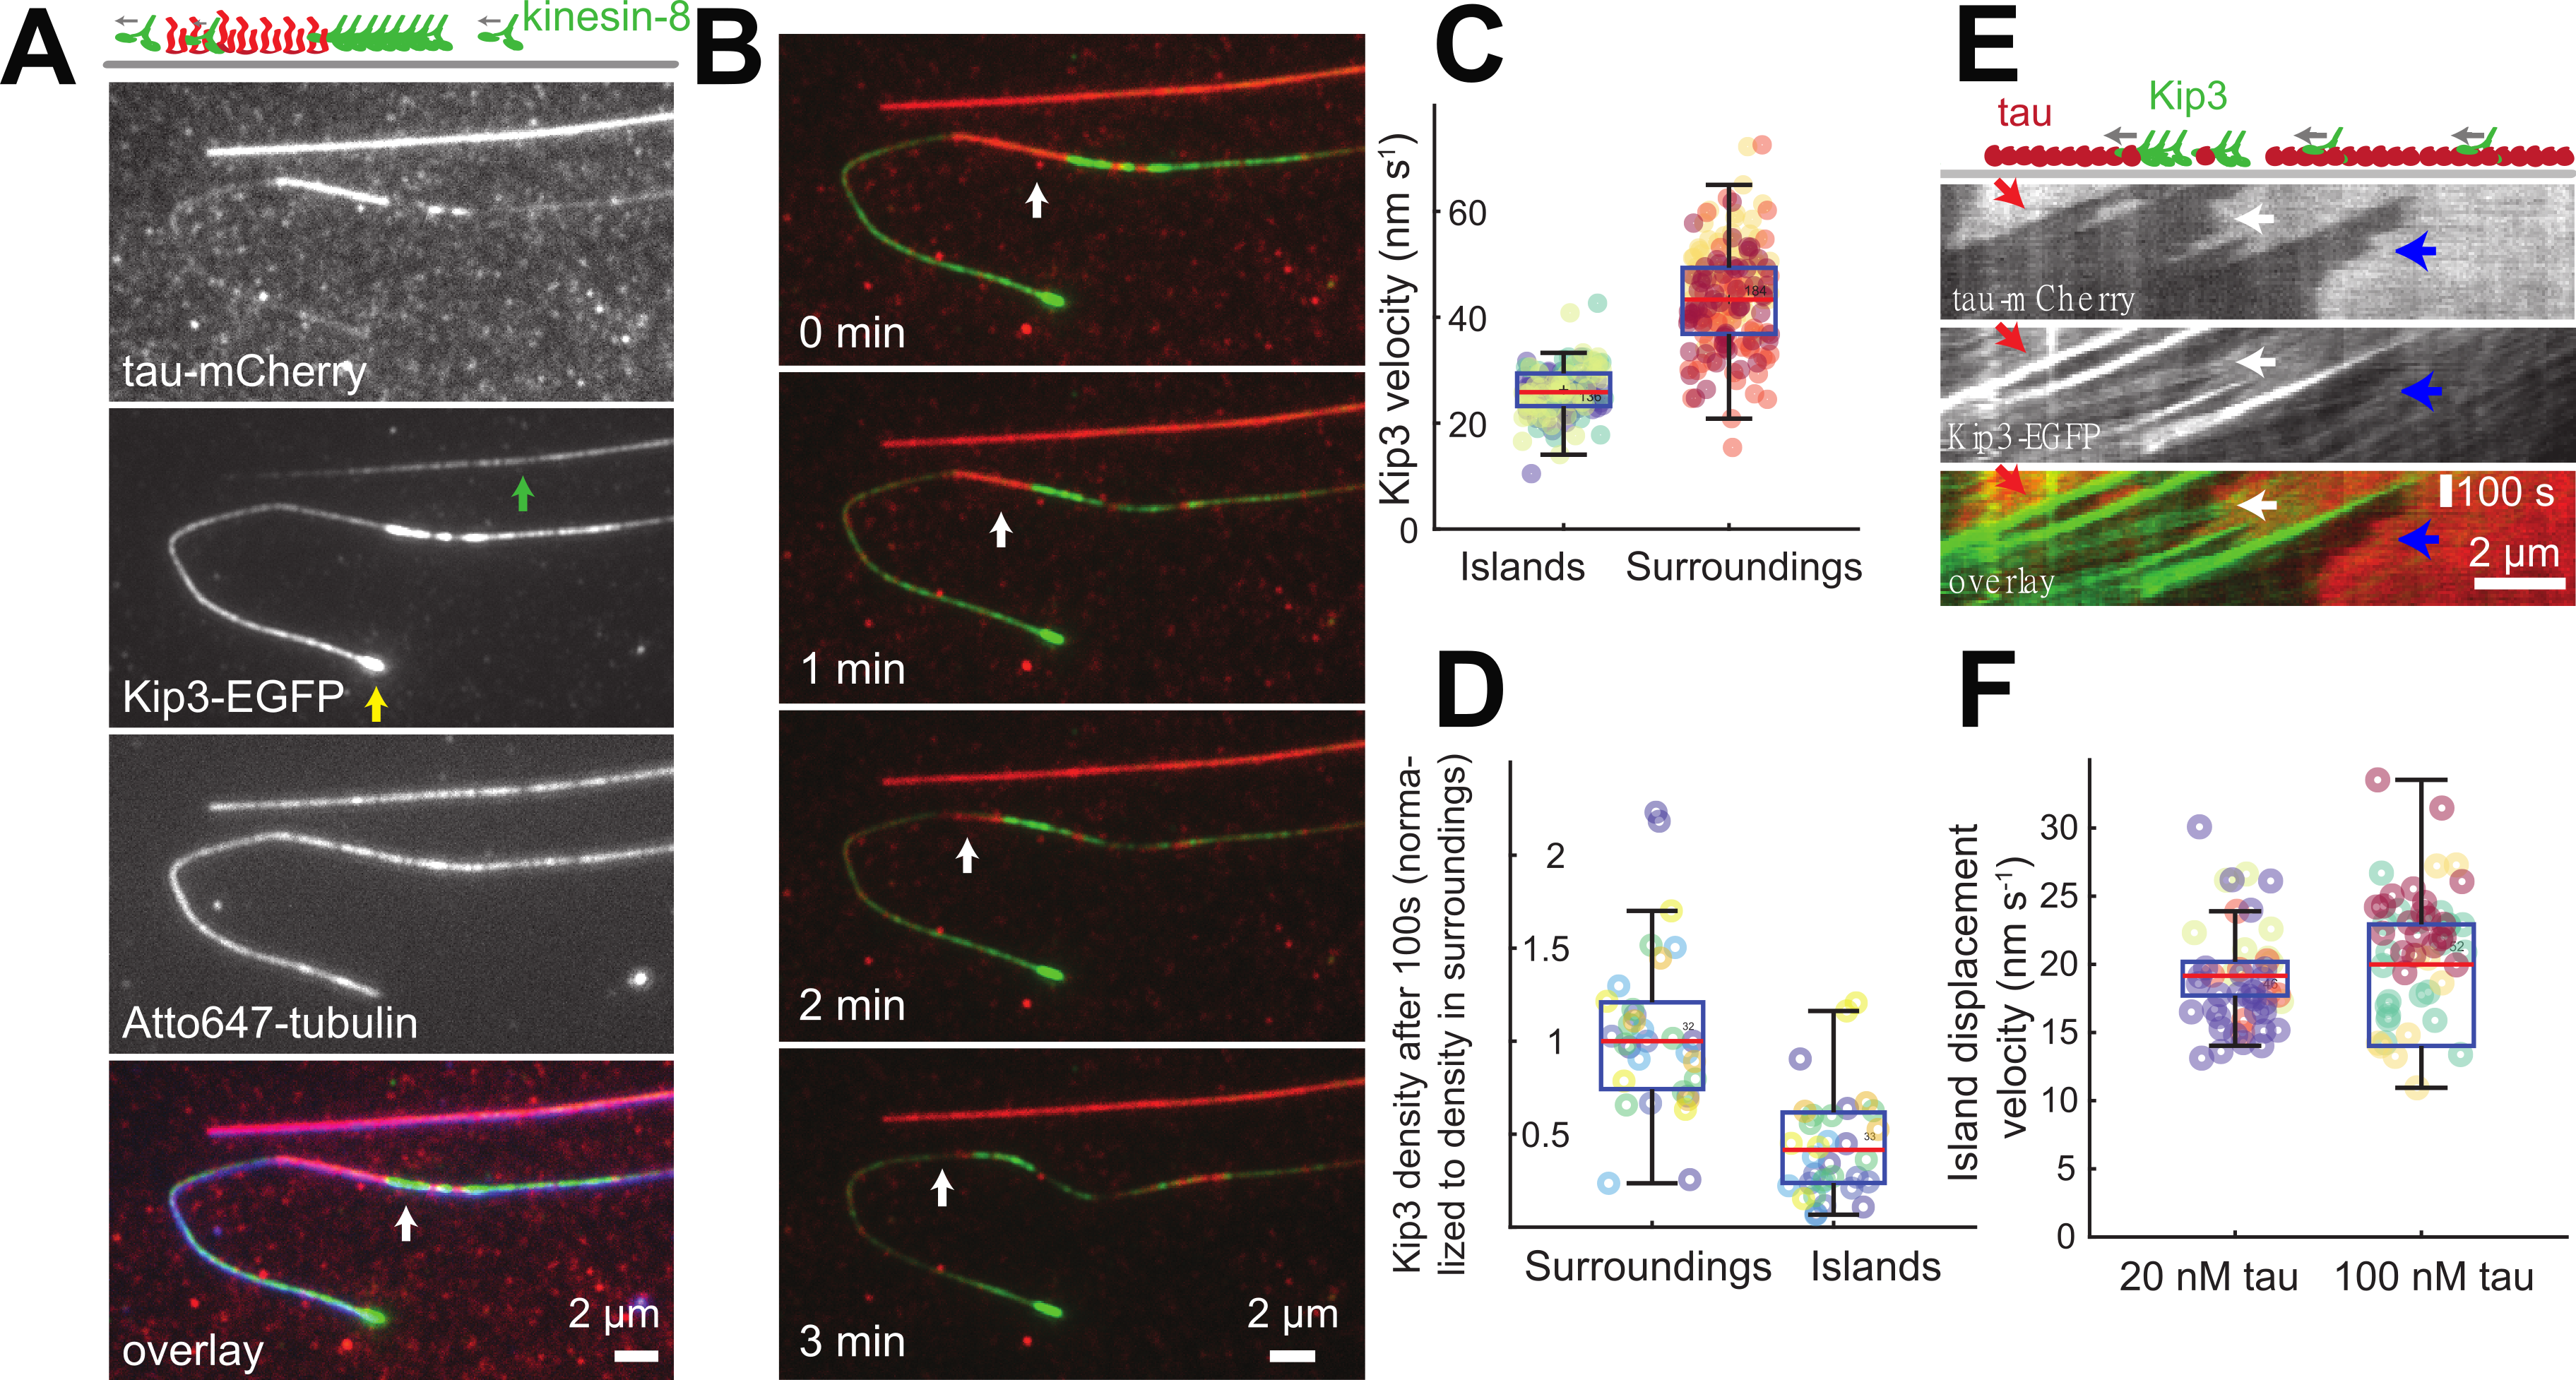
\includegraphics[width=1\linewidth]{Figures/taukip3.png}
\caption[Tau islands can be regulated by super-processive kinesin motors.]{
\textbf{Tau islands can be regulated by super-processive kinesin motors.} (A) Multichannel fluorescence micrographs showing Kip3 (kinesin-8, green) localizing outside and within the tau (red) islands (biggest island indicated by green arrow) on Atto-647-labeled microtubules (blue). An accumulation of Kip3 at an microtubule end is highlighted by an yellow arrow, an accumulation in front of an island by a white arrow. (B) Multicolor timelapse micrographs of the event shown in A documenting the removal of a tau island by Kip3 accumulating in front of it, where the receding of the island boundary is indicated by white arrow. (C) The measured velocities of single Kip3 motors moving inside and outside the islands at 10 nM tau in solution (3 experiments). (D) The measured Kip3 density inside and outside the islands 100 seconds after the addition of Kip3 (6 experiments). (E) Multichannel fluorescence kymograph showing a different event than A and B. The red arrows indicate an accumulation of Kip3 in front of an island, disassembling it. The white arrows indicate an instance where Kip3 molecules can clearly been observed to speed up as they leave the island. The blue arrows (added for this thesis) show a region of tau island "growing back" after having been disassembled. (F) Velocities of Kip3-GFP-driven disassembly of tau islands established at two different tau concentrations (3 experiments). Panels from \cite{Siahaan2019a}.
	}\label{taukip3}
\end{figure}

Kinesin-8, in contrast to kinesin-1, is a super-processive motor \pref{sec:kip3}{}, which led us to hypothesize that its interaction with tau islands might differ from the behavior by kinesin-1. For our experiments, we used S. cerevisiae Kip3, the best described member of the kinesin-8 family \pref{sec:kip3}{}. After the addition of 45nM (GFP-labeled) Kip3 to microtubules in the presence of 20nM or 100nM (mCherry-labeled) tau, we observed that Kip3 molecules could move in the low-density tau regions, like kinesin-1 \pref{taukip3}{A,B}. However, in contrast to kinesin-1, and presumably related to its characteristic of super-processivity, Kip3 could also traverse tau islands, albeit at a decreased velocity \pref{taukip3}{A-C}. Similarly, we also observed Kip3 to be less prevalent in regions covered by tau islands, indicating a lower affinity for these regions \pref{taukip3}{A,D}. We also observed the previously described \pref{sec:kip3}{} traffic jams at the end of microtubules \pref{taukip3}{A,B}. Interestingly however, we also observed that Kip3 accumulated, in the direction of its movement, at the boundaries of tau islands \pref{taukip3}{A,B}. Such Kip3 traffic jams evidently caused enhanced unbinding of tau at these positions, eventually leading to a disassembly of the islands from their boundaries with a velocity slightly lower than the velocity of Kip3 within islands \pref{taukip3}{B,C,E,F}. Notably, tau islands which had been removed in this way typically regrew after the Kip3 accumulates had passed \pref{taukip3}{E}. The island displacement by Kip3 shows that not only do tau islands regulate the interaction of other MAPs with the microtubule surface but that, vice versa, the activity of other MAPs, such as super-processive motors proteins, can regulate the dynamics of the islands themselves.

\FloatBarrier
\subsection{Highly curved microtubule regions displayed unique MAP interaction patterns}
\begin{figure}[h!]
\centering
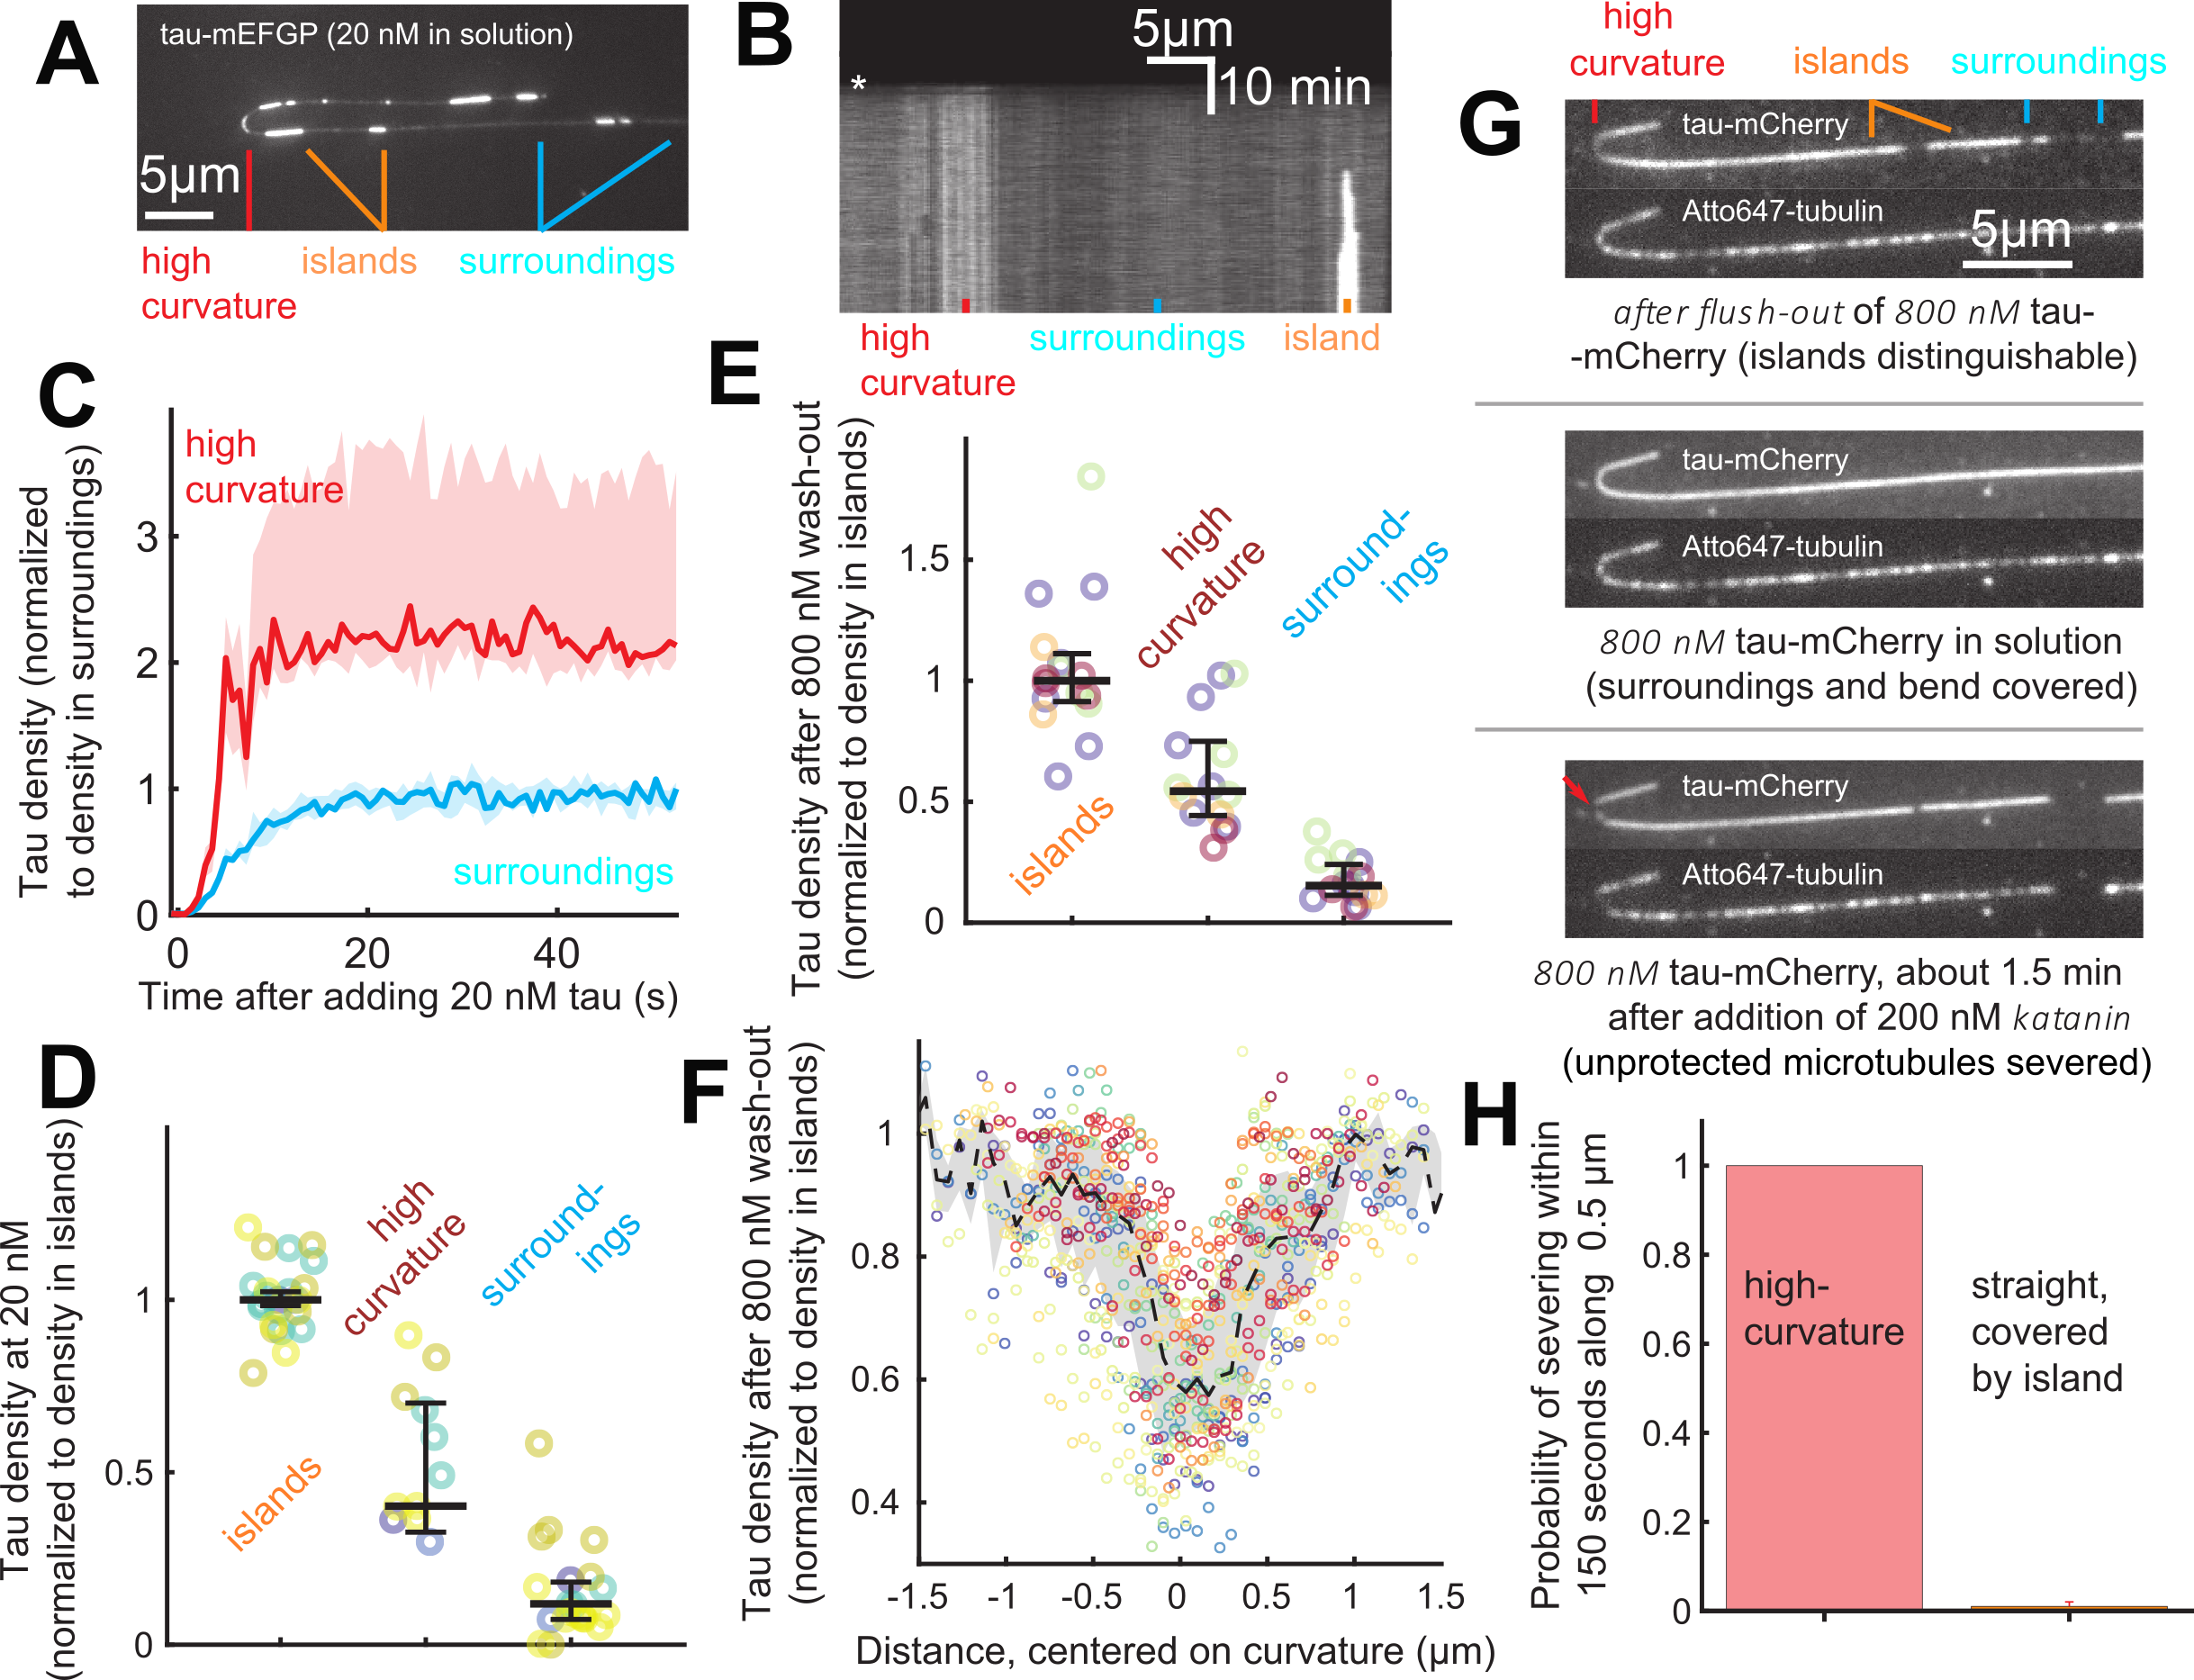
\includegraphics[width=1\linewidth]{Figures/taucurve.png}
\caption[Tau islands do not form at microtubule regions with high curvature.]{
\textbf{Tau islands do not form at microtubule regions with high curvature.} (A) Fluorescence micrograph showing the tau distribution on a highly curved microtubule at 20 nM tau in solution. (B) Kymograph showing the change in tau density along a highly curved region of a microtubule as well as the assembly of an island upon the addition of tau in solution. (C) Exemplary time-trace of the three different types of regions as shown in A and B after addition of 20 nM tau-mEGFP in solution (n = 5 microtubules). (D) Normalized steady-state densities measured in these three region types at 20 nM tau in solution (n = 11 high-curvature regions in 5 experiments). Points are color-coded by experiments, weighted such that each experiment has equal weight. (E) Normalized densities measured in the three region types around 1 minute after the removal of 0.8 µM tau from solution. Points are
color-coded by experiments (n = 15 high-curvature regions in 4 experiments), weighted such that each experiment has equal weight. (F) Tau density profiles along highly curved microtubule regions around 1 minute after removing 800 nM tau from solution. X-axis is centered on the point of highest curvature. Data are color-coded by microtubule and the density is normalized to the 90th percentile of the density-values of the respective microtubule. The red line represents the median of n = 30 microtubules (7 experiments). At 800 nM tau, there always were islands adjacent to microtubule bends, which is why the tau density to the left and right of the curved microtubule region is high even though tau has been removed from solution. A clear decrease in the tau density is apparent at the point of highest curvature. (G) Tau on microtubules after removing 800 nM tau from solution (upper panel); the same microtubule when having reintroduced 800 nM tau in solution (middle panel); the same microtubule shortly after 200 nM katanin have been added to the solution. The red arrow highlights cut in the high curvature region. (H) Probability of severing of highly curved microtubule regions and adjacent straight island-covered microtubule regions, within 150 s after adding katanin. The bars represent the probability averaged over n = 4 experiments (29 bends and 82 straight microtubules), error bars represent the S.D. Curved microtubule regions were always severed. In panels C-F, horizontal lines/lines/shaded areas represent the three quartiles. Panels from \cite{Siahaan2019a}.
	}\label{taucurve}
\end{figure}
In our assays, we noticed that at low tau concentrations, tau preferentially localized to highly-curved microtubules compared to regions outside of islands \pref{taucurve}{A-C}, as had previously been reported \parencite{Samsonov2004}. To be more precise, we observed that regions of highly curved microtubules (radius < 2.5 µm) exhibited a tau density that was higher than in the surroundings, but lower than in tau islands \pref{taucurve}{D}. In contrast to the islands, there was no growth from boundaries. Instead, in the high-curvature regions the tau density increased immediately after the addition of tau in solution, similar to the behavior in the regions surrounding the islands \pref{taucurve}{C}. Indeed, we observed very similar timescales of binding till saturation (6 ± 2 s for high-curvature regions, 8 ± 6 s for surroundings, weighted average ± S.D., 5 experiments). Moreover, the tau bound to highly curved microtubule regions also did not unbind as quickly as in the surroundings \pref{taucurve}{E,G upper panel}. Not only were these highly curved regions different from islands, we also never observed islands to form in such regions. This was the case even at 800nM tau in solution, where the regions adjacent to highly curved regions were (interestingly) always covered with islands \par{taucurve}{F}. Taken together, these findings indicate that tau cannot bind in a cooperative manner to highly curved microtubule regions. We thus hypothesized that highly curved microtubule regions would never be protected from katanin severing. This was indeed the case \pref{taucurve}{G,H}